\begin{figure}[!ht]
	\centering
	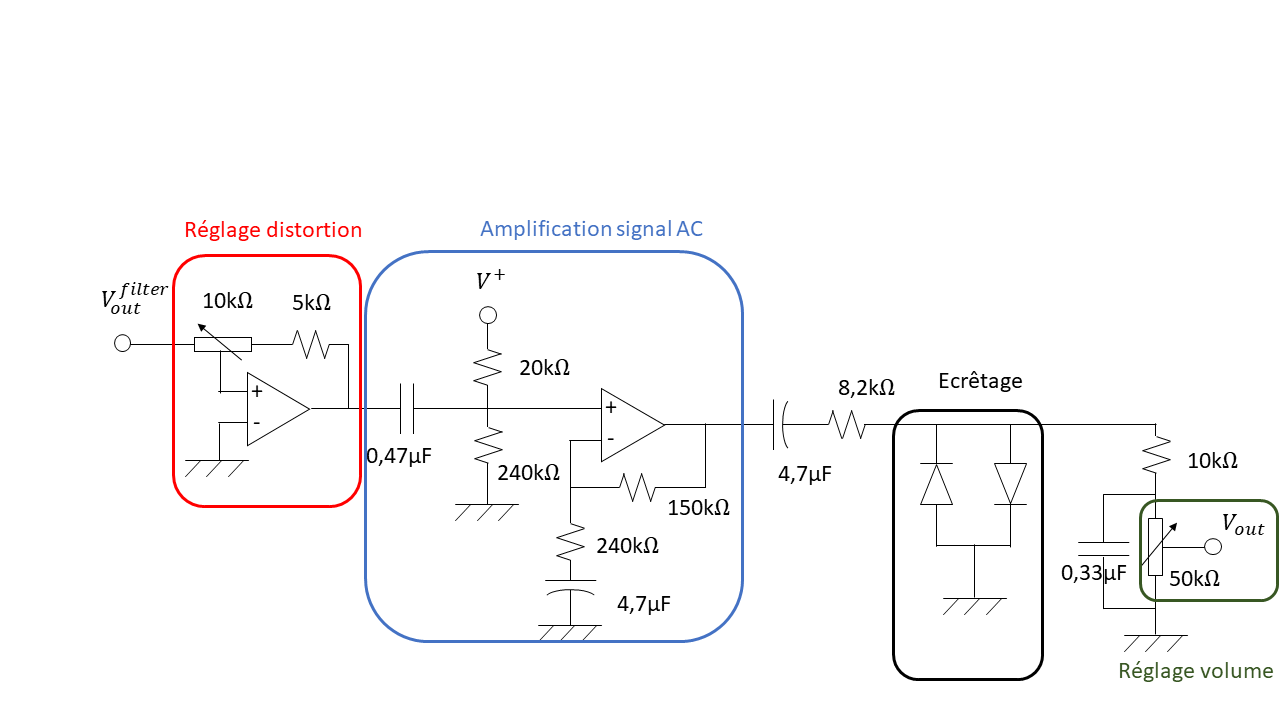
\includegraphics[width=.8\textwidth]{schematics-2}
	\caption{Schématique du bloc de distorsion et de contrôle du volume.}
	\label{fig3:clipper}
\end{figure}

Le circuit clipper permet d'introduire une distorsion dans le signal. Pour ce faire, les sinusoïdes sont remplacées par un signal carré. Le résultat sonore rajoute des grésillements au son original un peu comme sur une guitare électrique. Ce module est constitué des 4 éléments.  Les deux premiers sont utilisés afin d'amplifier le signal à distordre. Plus le signal entrant est amplifié, plus l'impact de la distorsion sera grand. En quelques mots, le bloc "réglage de distorsion" permet de régler via un potentiomètre l'amplification du signal et donc l'effet de la distorsion. Le bloc suivant permet d'amplifier uniquement la composante alternative de ce signal.

C'est le bloc "écrêtage" qui introduit la distorsion à l'aide de deux diodes. Ces diodes se comportent comme des courts circuits une fois une certaine tension à leurs bornes atteintes. Simplement, lorsque le signal d'entrée est supérieur à leur tension de seuil, la diode de droite devient passante avec la tension de seuil à ces bornes. Dans le cas d'un signal négatif inférieur à la tension de seuil, c'est la diode de gauche qui devient passante. Au final, les sinusoïdes à l'entrée de ce module sont transformées en signal carré. Le dernier bloc permet de régler le volume via un diviseur résistif.

Les Figures \ref{fig:ecret_pos} et \ref{fig:ecret_neg} donnent une idée de l'effet des diodes sur l'alternance positive et négative respectivement.

\begin{minipage}[c]{.49\textwidth}
	\centering
	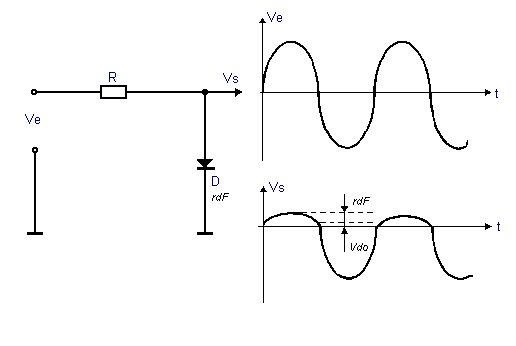
\includegraphics[width=\textwidth]{figures/ecret_pos.png}
	\captionof{figure}{Écrêtage de l'alternance positive.}
	\label{fig:ecret_pos}
\end{minipage}
\hfill
\begin{minipage}[c]{.49\textwidth}
	\centering
	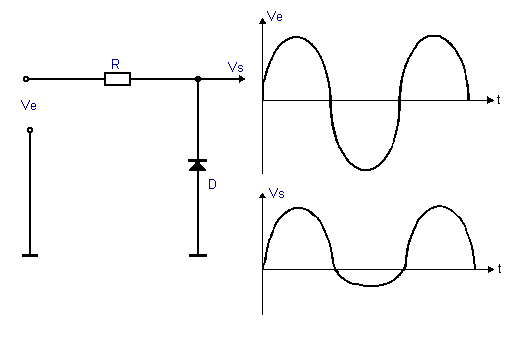
\includegraphics[width=\textwidth]{figures/ecret_neg.png}
	\captionof{figure}{Écrêtage de l'alternance négative.}
	\label{fig:ecret_neg}
\end{minipage}
\vspace{1cm}